% Frugal AI seminar, part 4: how small models work. File sizes are from the Hugging Face listing named in the
% Ref line; other figures from the cited papers (their claims, on their setups). CheatSheet-safe: no floats.

\section[Models]{How Small Models Work}

%%%%%%%%%%%%%%%%%%%%%%%%%%%%%%%%%%%%%%%%%%%%%%%%%%%
\begin{frame}[fragile]\frametitle{}
\begin{center}
{\Large How Small Models Work}

\medskip
{\small (Shrinking a model without throwing it away)}
\end{center}
\end{frame}

%%%%%%%%%%%%%%%%%%%%%%%%%%%%%%%%%%%%%%%%%%%%%%%%%%%
\begin{frame}[fragile]\frametitle{What Is a Small Model?}
\begin{itemize}
\item In this talk: roughly 0.5 to 4 billion parameters, small enough to run on a laptop CPU.
\item Two models used in the examples: \textbf{Qwen3 1.7B} (Apache-2.0 licence) and \textbf{Gemma 2 2B} (Google's Gemma terms of use; about 2.6 billion parameters, which the model card's metadata rounds to 3 billion).
\item Small does not mean toy. It means: pick the job first, then the smallest model that does it well enough, and measure that on your own task.
\item The rest of this part: four ways models are made small or cheap.
\end{itemize}
{\tiny (Ref: Hugging Face model cards for Qwen/Qwen3-1.7B and google/gemma-2-2b-it)}
\end{frame}

%%%%%%%%%%%%%%%%%%%%%%%%%%%%%%%%%%%%%%%%%%%%%%%%%%%
\begin{frame}[fragile]\frametitle{Quantisation: Fewer Bits per Weight}
\begin{center}
\adjustbox{max width=0.78\linewidth, max totalheight=0.50\textheight}{\includegraphics{frugal_gemma_sizes}}
\end{center}
\begin{itemize}
\item Quantisation stores each weight in fewer bits. The same Gemma 2 2B goes from 10.5 GB (full precision) to 1.71 GB (4-bit Q4\_K\_M): about 6 times smaller.
\item What you lose depends on the model and the task. Measure it on yours.
\end{itemize}
{\tiny (Ref: Hugging Face, lmstudio-community/gemma-2-2b-it-GGUF, file sizes)}
\end{frame}

%%%%%%%%%%%%%%%%%%%%%%%%%%%%%%%%%%%%%%%%%%%%%%%%%%%
\begin{frame}[fragile]\frametitle{A 2B Model Against a Microcontroller}
\begin{center}
\adjustbox{max width=0.82\linewidth, max totalheight=0.45\textheight}{\includegraphics{frugal_size_vs_memory}}
\end{center}
\begin{itemize}
\item The 1.71 GB model file is about 6,700 times the 256 KB of RAM on an Arduino Nano 33 BLE Sense. A language model does not fit there; small classifiers do.
\item A Raspberry Pi 5 comes with 1 to 16 GB of RAM, and an 8 GB laptop is enough: those are the language-model platforms.
\end{itemize}
{\tiny (Ref: Nordic nRF52840; Raspberry Pi 5 product page; AIOOLL README; decimal units)}
\end{frame}

%%%%%%%%%%%%%%%%%%%%%%%%%%%%%%%%%%%%%%%%%%%%%%%%%%%
\begin{frame}[fragile]\frametitle{Distillation: Teacher and Student}
\begin{center}
\adjustbox{max width=0.85\linewidth, max totalheight=0.26\textheight}{%
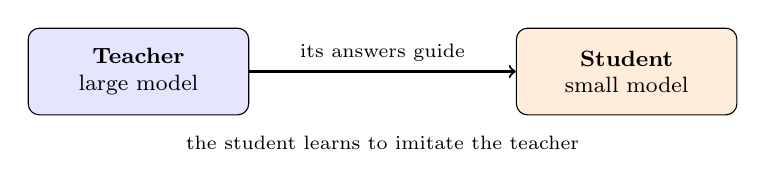
\begin{tikzpicture}
\tikzstyle{b}=[draw, rounded corners, align=center, minimum height=1.1cm, minimum width=2.8cm, font=\footnotesize]
\node[b, fill=blue!10] (t) at (0,0) {\textbf{Teacher}\\large model};
\node[b, fill=orange!15] (s) at (6.2,0) {\textbf{Student}\\small model};
\draw[->, thick] (t) -- node[above, font=\scriptsize] {its answers guide} (s);
\node[font=\scriptsize] at (3.1,-0.9) {the student learns to imitate the teacher};
\end{tikzpicture}}
\end{center}
\begin{itemize}
\item Train a small \textbf{student} model to imitate a large \textbf{teacher}, so the student keeps most of the skill in far fewer parameters.
\item Example: MoScNet, which reads Modi script. Its authors report a student about 163 times smaller in parameters than its teacher that outperforms it, on their dataset.
\item Distillation is how many small models get good: the large model's work is reused, not repeated.
\end{itemize}
{\tiny (Ref: Kausadikar et al., arXiv 2503.13060)}
\end{frame}

%%%%%%%%%%%%%%%%%%%%%%%%%%%%%%%%%%%%%%%%%%%%%%%%%%%
\begin{frame}[fragile]\frametitle{Memory: The KV Cache}
\begin{itemize}
\item While generating, a model keeps the keys and values of every token it has seen (the KV cache) so it need not recompute them.
\item A serving paper states that this memory for each request ``is huge and grows and shrinks dynamically''.
\item So long prompts cost memory as well as time: lean context is a frugal practice, not only a tidy one.
\end{itemize}
{\tiny (Ref: Kwon et al., PagedAttention, arXiv 2309.06180)}
\end{frame}

%%%%%%%%%%%%%%%%%%%%%%%%%%%%%%%%%%%%%%%%%%%%%%%%%%%
\begin{frame}[fragile]\frametitle{Mixture of Experts}
\begin{itemize}
\item A router picks a few expert blocks for each token instead of using the whole network.
\item Mixtral has 8 experts per layer and uses 2 per token: 47 billion parameters in total, 13 billion active for each token.
\item Watch the catch: all the weights must still sit in memory, so this saves compute more than memory. It is not automatically a fit for small devices.
\end{itemize}
{\tiny (Ref: Jiang et al., Mixtral of Experts, arXiv 2401.04088)}
\end{frame}

%%%%%%%%%%%%%%%%%%%%%%%%%%%%%%%%%%%%%%%%%%%%%%%%%%%
\begin{frame}[fragile]\frametitle{Frozen Encoder Plus a Small Head}
\begin{center}
\adjustbox{max width=0.9\linewidth, max totalheight=0.22\textheight}{%
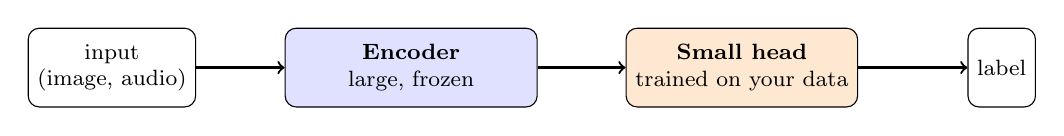
\begin{tikzpicture}
\tikzstyle{b}=[draw, rounded corners, align=center, minimum height=1cm, font=\footnotesize]
\node[b] (x) at (0,0) {input\\(image, audio)};
\node[b, fill=blue!12, minimum width=3.2cm] (e) at (3.8,0) {\textbf{Encoder}\\large, frozen};
\node[b, fill=orange!18, minimum width=2.6cm] (h) at (8,0) {\textbf{Small head}\\trained on your data};
\node[b] (y) at (11.3,0) {label};
\draw[->, thick] (x) -- (e); \draw[->, thick] (e) -- (h); \draw[->, thick] (h) -- (y);
\end{tikzpicture}}
\end{center}
\begin{itemize}
\item Train a large encoder once, then keep it frozen and train only a small head on top for your task.
\item V-JEPA 2's paper evaluates this way, with a small attention-based probe on a frozen encoder; LeJEPA reports 79\% on ImageNet-1k with a frozen backbone and a linear probe (the authors' claim).
\item Why it is frugal: only the small head needs your data and compute. The catch: the encoder still has to run at inference, so it is not free on small hardware.
\end{itemize}
{\tiny (Ref: Assran et al., arXiv 2506.09985; Balestriero and LeCun, arXiv 2511.08544)}
\end{frame}
